\section{Feature editing}

To explore the possibility of generating different facial expressions and features, we explored how different images are generated. Since the model uses StyleGAN2, it also makes use of the latent vector determining the generated image \cite{StyleGAN2}. This vector contains 512 scalar entries. To explore how each entry changes the image, we changed one entry of the latent vector at a time with five different values to explore the entire range of the scalar. The results can be seen in figure \ref{fig:changing_latent}. Although each entry of the latent vector are normally drawn from a normal distribution with standard deviation of 1, we choose to make the changes bigger in a range of [-10, 10] to show the change of the single entry more. We notice that at the extremes, the original person has completely changed into somebody else. This lead us to the exploration of the amount of truly different faces that can be generated by this model - not just the small changes such as glasses or hair length. Each latent vector entry can change the original face towards two new faces. Therefore, the amount of faces that could be generated by the model exceeds $2^{512} \approx 10^{124}$.

\begin{figure}[H]
    \centering
    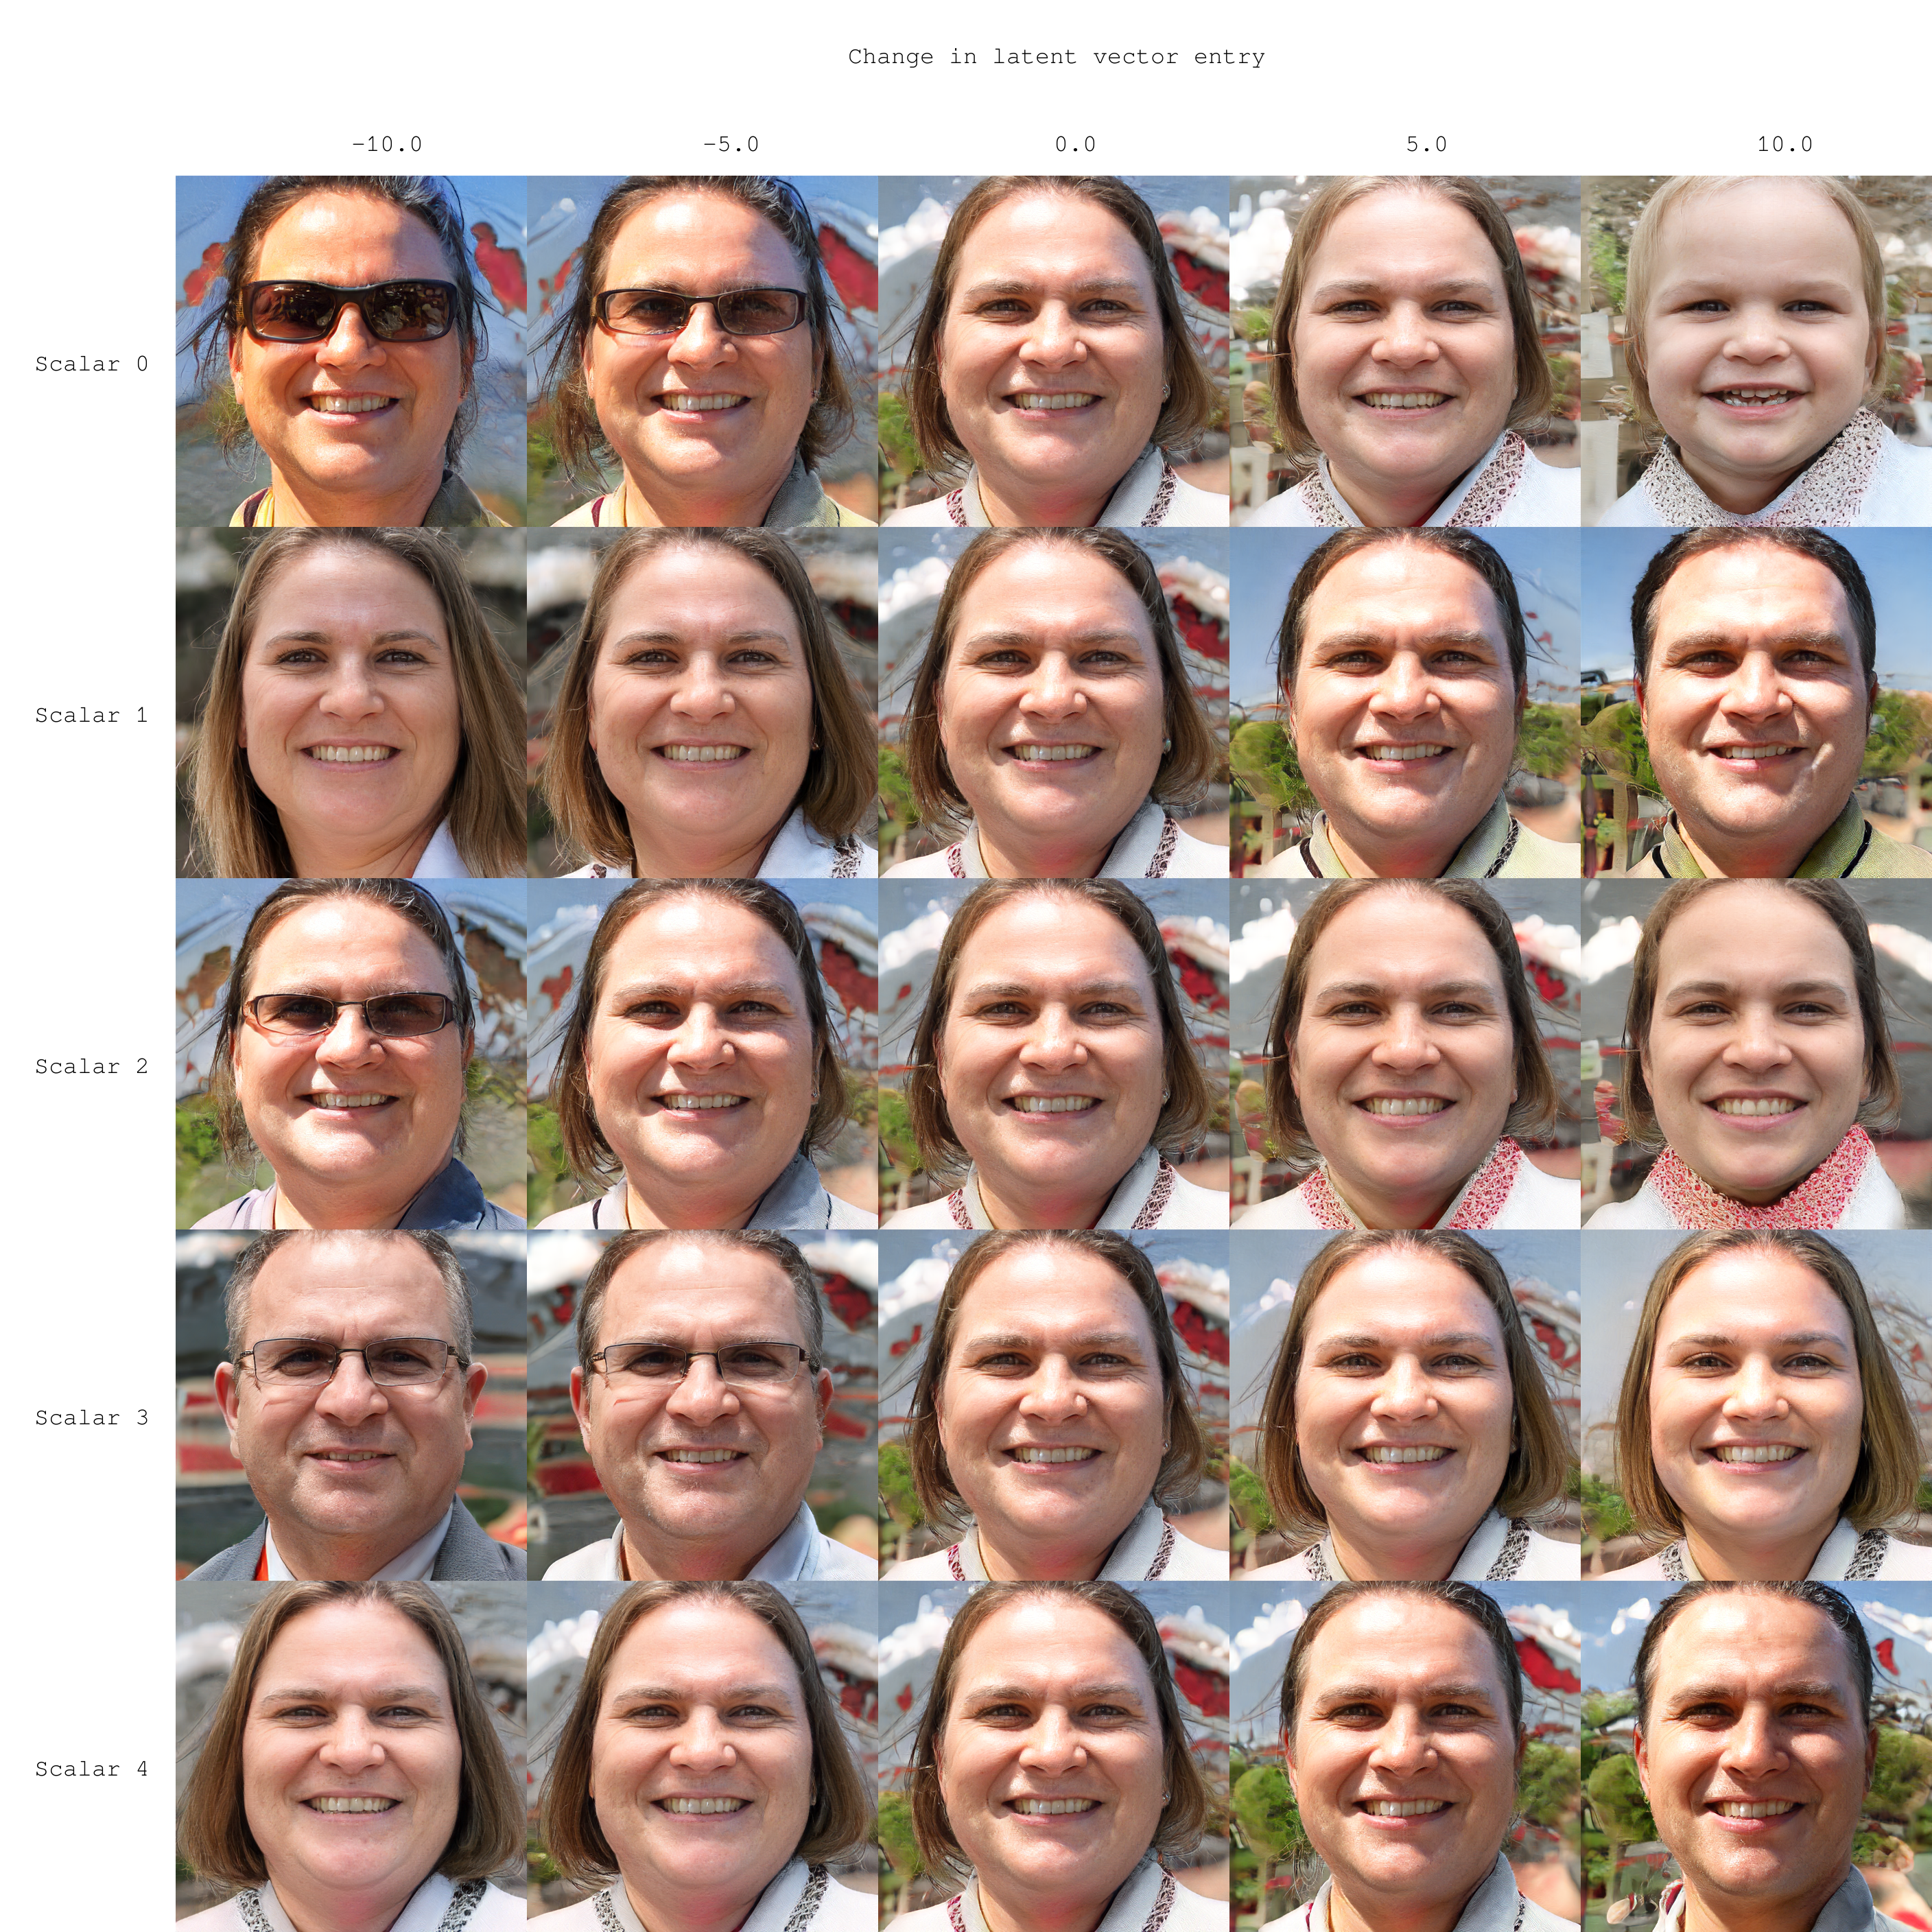
\includegraphics[width=0.9\linewidth]{latent-0004-ffhqrebalanced512-64.png}
    \caption[width=0.6]{Generated images for change in single latent vector entry. Showing the possibility to change the original image features towards different facial and background features}
    \label{fig:changing_latent}
\end{figure}